\documentclass[border=0.8ex,svgnames,varwidth]{standalone}
\usepackage{amsmath,mathtools}
\usepackage{fontspec}
\setmainfont{Source Serif 4}
\setsansfont{Source Sans 3}
\setmonofont{Source Code Pro}
\usepackage{ifthen}
\usepackage{subcaption}
\usepackage{tikz}
\usetikzlibrary{chains,shapes.multipart,calc}
\makeatletter
\let\widthof=\pgfmath@calc@widthof%
\let\heightof=\pgfmath@calc@heightof%
\let\depthof=\pgfmath@calc@depthof%
\makeatother
\captionsetup{
  font=scriptsize,
  labelfont=it,
  textfont=rm,
  labelformat=parens,
  position=above,
  labelsep=space,
  justification=centering,
}
\begin{document}
\begin{figure}
  \centering
  \begin{subfigure}[t]{\linewidth}
    \centering
    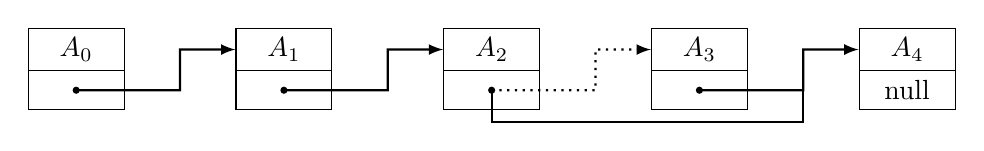
\begin{tikzpicture}
      \begin{scope}[
        every node/.style={
          draw,
          on chain,
          text centered,
          text width=2.8em,
          rectangle split,
          rectangle split parts=2,
          rectangle split every empty part={},
          rectangle split part align={center,center},
          rectangle split empty part width=\widthof{null},
          rectangle split empty part height=\heightof{null},
          rectangle split empty part depth=\depthof{null},
        },
        node distance=4em,
        start chain,
        ]
        \foreach \i in {0,...,3}{
          \node(a\i){\nodepart{one} \(A_{\i}\)};
        }
        \node(a4) {\nodepart{one} \(A_{4}\) \nodepart{two} null};
      \end{scope}
      \begin{scope}[every path/.style={draw,thick,>=latex}]
        \foreach \i in {0,...,3}{
          \pgfmathtruncatemacro{\x}{\i+1};
          \coordinate(a\i-center) at (a\i.two west-|a\i.two south);
          \coordinate(a\i-next) at ($(a\i.two east)!0.5!(a\x.two west)$);
          \ifthenelse{\x=3}{
            \pgfmathtruncatemacro{\y}{\x+1};
            \coordinate(a\x-next) at ($(a\x.two east)!0.5!(a\y.two west)$);
            \path[->,dotted] (a\i-center) -- (a\i-next) |- (a\x.one west);
            \path (a\i-center) -- ($(a\i.south)+(0,-1ex)$) -| (a\x-next)
            ++(0,1ex);
          }{
            \path[->] (a\i-center) -- (a\i-next) |- (a\x.one west);
          };
          \fill (a\i.two west-|a\i.two south) circle (0.2ex);
        }
      \end{scope}
    \end{tikzpicture}
    \caption{delete}
  \end{subfigure}
  \bigskip
  \begin{subfigure}[t]{\linewidth}
    \centering
    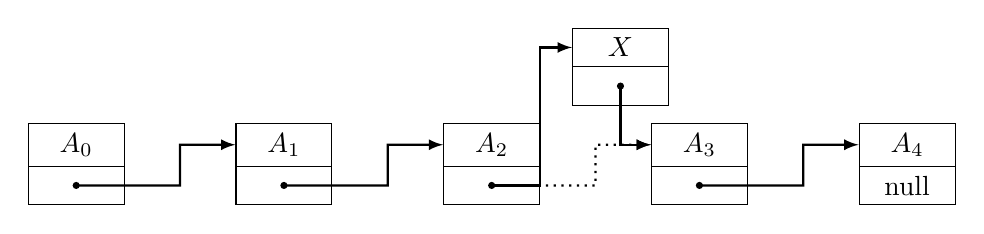
\begin{tikzpicture}
      \begin{scope}[
        every node/.style={
          draw,
          on chain,
          text centered,
          text width=2.8em,
          rectangle split,
          rectangle split parts=2,
          rectangle split every empty part={},
          rectangle split part align={center,center},
          rectangle split empty part width=\widthof{null},
          rectangle split empty part height=\heightof{null},
          rectangle split empty part depth=\depthof{null},
        },
        node distance=4em,
        start chain,
        ]
        \foreach \i in {0,...,3}{
          \node(a\i){\nodepart{one} \(A_{\i}\)};
          \ifthenelse{\i=3}{
            \pgfmathtruncatemacro{\x}{\i-1};
            \node[above=2.1em of $(a\i)!0.38!(a\x)$](a-new){\nodepart{one} \(X\)};
            \chainin(a\i);
          }{};
        }
        \node(a4) {\nodepart{one} \(A_{4}\) \nodepart{two} null};
      \end{scope}
      \begin{scope}[every path/.style={draw,thick,>=latex}]
        \foreach \i in {0,...,3}{
          \pgfmathtruncatemacro{\x}{\i+1};
          \coordinate(a\i-center) at (a\i.two west-|a\i.two south);
          \coordinate(a\i-next) at ($(a\i.two east)!0.5!(a\x.two west)$);
          \ifthenelse{\i=2}{
            \path[->,dotted] (a\i-center) -- (a\i-next) |- (a\x.one west);
            \path[->] (a\i-center) -- (a\i.two east) |- (a-new.one west);
          }{
            \path[->] (a\i-center) -- (a\i-next) |- (a\x.one west);
          };
          \fill (a\i-center) circle (0.2ex);
        }
        \coordinate(a-new-center) at (a-new.two west-|a-new.two south);
        \path[->] (a-new-center) |- (a3.one west);
        \fill (a-new-center) circle (0.2ex);
      \end{scope}
    \end{tikzpicture}
    \caption{insert}
  \end{subfigure}
\end{figure}
\end{document}
